\documentclass[14pt]{article}

\usepackage{amsmath, amsthm, amssymb}
\DeclareMathOperator*{\argmax}{arg\,max}
\DeclareMathOperator*{\argmin}{arg\,min}
\usepackage{graphicx, verbatim}
\usepackage{multirow}
\usepackage[margin = 1in]{geometry}
\usepackage[dvipsnames]{xcolor}
\setlength{\parindent}{0pt}
\DeclareRobustCommand{\stirling}{\genfrac\{\}{0pt}{}}

\usepackage{array}
\newcolumntype{R}[1]{>{\raggedleft\arraybackslash}p{#1}}

\usepackage{tikz}
\usetikzlibrary{automata,positioning}

\newenvironment{blockcode}
{\leavevmode\color{Violet}\verbatim}{\endverbatim}


\begin{document}

\Css{body{margin: 75px 300px 100px;
		  %font-family: Arial, Helvetica, sans-serif;
		  font-size: 18px;
		  background-color: WhiteSmoke;}} 
\begin{center}
\section*{Expectation-Maximization Algorithm}

\subsection*{Background}
\end{center}

In statistics and its applications, maximum likelihood estimation (MLE) is a popular technique for estimating the parameters of a distribution from observed data. The likelihood function on a parameter $\theta$ given data $y$ is equivalent to the probability density function of $y$ with parameter $\theta$.

$$L(\theta|y) = f(y|\theta)$$

The maximum likelihood estimator of $\theta$ is the argmax of the likelihood function.  Intuitively, it can be thought of as the parameter that is most likely to have generated the data.  In practice, it is conveneient to instead maximize the log of the likelihood function, $\ell(\theta|y)$.

However, there are many situations where the not all information is available, and our data has a hidden (or latent) component.  In this situation, finding the MLE of the parameters using only the observed data can be difficult or even intractable.  The Expectation-Maximizztion (E-M) algorithm, introduced in 1977, is an iterative method for obtaining the MLE when there is latent or missing data.

\begin{center}
\subsection*{Algorithm}
\end{center}

The E-M works by alternating between estimating the latent data and the parameters at each step.  The data is used to estimate the parameters, then the parameters are used to estimate the data, and so on until convergence.

Let $X$ be our observed data, $Z$ be our latent data, and $\theta$ our parameter of interest.  The E-M algorithm is as follows:
\begin{enumerate}
\item Initialize $\theta$ to some starting value(s).
\item \textbf{E-Step:} At time $t$, estimate the values of the latent data $Z$ based on the current value of $\theta$.  This gives an expression to update $\theta$ based on the expected value of the log-likelihood with respect to the new conditional distribution of $Z$ given $X$. 
$$Q(\theta|\theta^{(t)}) = E_{Z|X,\theta^{(t)}}[\ell(\theta|X, Z)]$$
\item \textbf{M-Step:} Find the most likely parameter(s) given the data from step 2.  This is equivalent to maximizing the quantity we defined before:
$$\theta^{(t+1)} = \argmax_{\theta}Q(\theta|\theta^{(t)})$$
\item Repeat steps 2 and 3 until convergence.
\end{enumerate}

\begin{center}
\subsection*{E-M and Hidden Markov Models}
\end{center}

One of the most important applications of the E-M algorithm in NLP is the task of training a Hidden Markov Model (HMM).  An HMM is based on a structure called a Markov chain, which is a sequence of probabilistic events, or states.  A Markov chain obeys the Markov assumption, which states that the probability of a state depends only on the previous state.  Equivalently, only the current state can be used to predict the next state.

An HMM is an extension of a Markov chain that assumes that all states in the chain are hidden.  However, the states emit observations with a certain probability.  We cannot see any of the states, but we can see the observations.  This model lends itself particularly well to the NLP task of part-of-speech (POS) tagging.  In this construction, words would be observations, and POS tags would be states.  Each POS tag would depend only on the previous tag.

\begin{figure}
\centering
\begin{center}
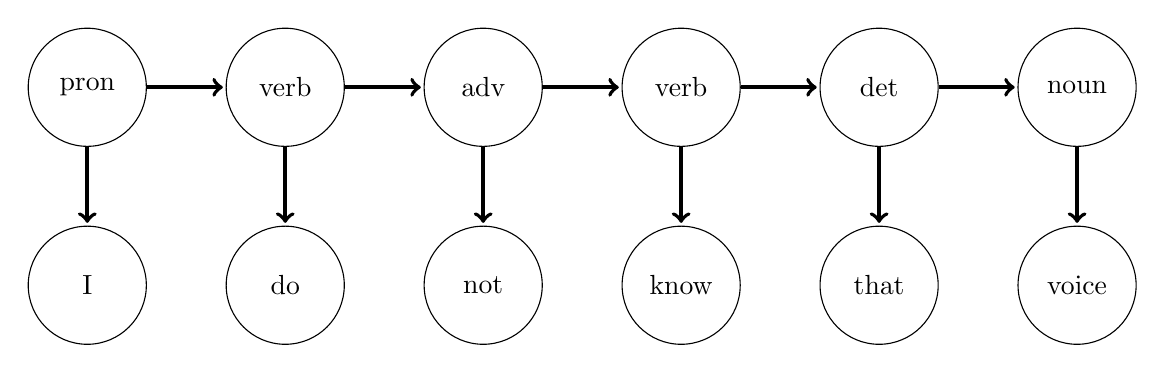
\begin{tikzpicture}
\node[state,minimum size=1.5cm] (pron) {pron};
\node[state, right=of pron,minimum size=1.5cm] (verbI) {verb};
\node[state, right=of verbI,minimum size=1.5cm] (adv) {adv};
\node[state, right=of adv,minimum size=1.5cm] (verbII) {verb};
\node[state, right=of verbII,minimum size=1.5cm] (det) {det};
\node[state, right=of det,minimum size=1.5cm] (noun) {noun};

\node[state, below=of pron,minimum size=1.5cm] (I) {I};
\node[state, below=of verbI,minimum size=1.5cm] (do) {do};
\node[state, below=of adv,minimum size=1.5cm] (not) {not};
\node[state, below=of verbII,minimum size=1.5cm] (know) {know};
\node[state, below=of det,minimum size=1.5cm] (that) {that};
\node[state, below=of noun,minimum size=1.5cm] (voice) {voice};

\draw[every loop, line width=.5mm,]
(pron) edge node {} (I)
(verbI) edge node {} (do)
(adv) edge node {} (not)
(verbII) edge node {} (know)
(det) edge node {} (that)
(noun) edge node {} (voice)
(pron) edge node {} (verbI)
(verbI) edge node {} (adv)
(adv) edge node {} (verbII)
(verbII) edge node {} (det)
(det) edge node {} (noun);
\end{tikzpicture}\\
\caption{An HMM structure on an example sentence. States (POS tags) are on top, and observations (words) are below.}
\end{center}
\end{figure}

Formally, an HMM is defined as a set of five components:
\begin{itemize}
\item a set $Q$ of $N$ hidden states
$$Q = q_1,\ldots,q_N$$
\item an $N\times N$ transition probability matrix where $a_{ij}$ is the probability of transitioning from state $i$ to $j$ and $\sum_j\; a_{ij} = 1 \quad\forall i$
$$A = a_{11}\ldots a_{ij}\ldots a_{NN}$$
\item a sequence $V$ of $M$ possible observations
$$V = \{v_1, \ldots, v_M\}$$
\item an $N\times M$ matrix $B$ of observation likelihoods where $b_{ij}$ is the probability of state $i$ generating observation $j$ and $\sum_j\; b_{ij} = 1 \quad\forall i$
$$B = b_{11}\ldots b_{ij}\ldots b_{NM}$$
\item an initial probability distribution $\pi$ over states, where $\pi_i$ is the probability that the chain starts with state $i$, and $\sum_i\; \pi_i = 1$
$$\pi = \pi_1,\ldots,\pi_N$$
\end{itemize}

Given a set of possible states $Q$, a vocabulary $V$, and an unlabeled observation $O$, training an HMM requires training both the transition probability matrix $A$ and the obeservation matrix $B$.  This is a daunting task, but the E-M algorithm allows us to iteratively improve our estimates of these probabilities.  The \textbf{forward-backward}, or \textbf{Baum-Welch} algorithm is a specific instance of the E-M algorithm designed for this purpose.

\begin{center}
\subsection*{The Forward-Backward Algorithm}
\end{center}

The E-step of the forward-backward algorithm makes use of forward probabilities and backward probabilities, which are caculated from $A$, $B$, and a sequence of observations $O$ of length $T$ for a state $i$ and a time $t$.  Both are computed recursively.

The forward probability $\alpha_i(t)$ is the probability of seeing observations $o_1,o_2,\ldots,o_t$ and being in state $i$ at time $t$:
$$\alpha_i(1) = \pi_ib_i(o_1)$$
$$\alpha_i(t) = b_i(o_t)\sum_{j=1}^N \alpha_j(t-1)a_{ji}$$

So, the forward probability of $o_t$ for state $i$ is the observation probability of $o_t$ for state $i$ times the sum of the forward probabilities of the previous observation times the transition probability from $j$ to $i$ for all $j$ states.

The backward probability $\beta_i(t)$ is the probability of seeing the ending observations $o_{t+1},\ldots,o_T$ given starting state $i$ at time $T$:
$$\beta_i(T) = 1$$
$$\beta_i(t) = \sum_{j=1}^N \beta_j(t+1)a_{ij}b_j(y_{t+1})$$

So, the backward probability of $o_t$ is the sum of the backward probability of the next state times the transiiton probability from $j$ to $i$ times the observation probability of the next state for all $j$ states.

The forward and backward probabilities, as well as the current estimates for $A$ and $B$, allow us to calculate the final two quantities needed for the E-step, $\gamma_i(t)$ and $\xi_{ij}(t)$.

The quantity $\gamma_i(t)$ is the probability of being in state $i$ at time $t$ given $O$, $A$, and $B$:

$$\gamma_i(t) = \frac{\alpha_i(t)\beta_i(t)}{\sum_{j=1}^N \alpha_j(t)\beta_j(t)}$$

The quantity $\xi_{ij}(t)$ is the probability of being in state $i$ at time $t$ and being in state $j$ at time $t+1$ given $O$, $A$, and $B$:

$$\xi_{ij}(t) = \frac{\alpha_i(t)a_{ij}\beta_j(t+1)b_j(o_{t+1})}{\sum_{j=1}^N \alpha_j(t)\beta_j(t)}$$

The denominators in both $\gamma_i(t)$ and $\xi_{ij}(t)$ represent the probability of seeing the entire observation sequence $O$.

We can now use these two quantities to update $A$ and $B$ (and $\pi$) in the M-step.

$$\pi^*_i = \gamma_i(1)$$

$$a^*_{ij} = \frac{\sum_{t=1}^{T-1}\xi_{ij}(t)}{\sum_{t=1}^{T-1}\gamma_i(t)}$$

$$b^*_{ij} = \frac{\sum_{i=1}^T \gamma_i(t)\cdot I(o_t = v_k)}{\sum_{t=1}^T \gamma_i(t)}$$

where $I(o_t = v_k)$ is an indicator function that is 1 when $o_t = v_k$, and 0 otherwise.  To summarize, the full algorithm is:
\begin{enumerate}
\item Initialize $\pi, A,$ and $B$, either randomly or using prior information
\item \textbf{E-Step:} Calculate forward and backward probabilities for all states using the entire training sequence.  Use these, as well as $\pi, A,$ and $B$, to update $\gamma$ and $\xi$.
\item \textbf{M-Step:} Update $\pi, A,$ and $B$ using $\gamma$ and $\xi$.
\item Repeat steps 2 and 3 until convergence, e.g. the norms of the previous $A$ and $B$ are within $\epsilon$ of the norms of the current $A$ and $B$.
\end{enumerate}

\end{document}